\documentclass{article}
\usepackage{tmlr}
\usepackage{amsmath,amssymb,amsthm,mathtools}
\usepackage{booktabs}
\usepackage{graphicx}
\usepackage[colorlinks=true,linkcolor=blue,citecolor=blue,urlcolor=blue]{hyperref}
\usepackage{url}
\usepackage{microtype}

\newtheorem{theorem}{Theorem}[section]
\newtheorem{proposition}[theorem]{Proposition}
\newtheorem{lemma}[theorem]{Lemma}
\newtheorem{corollary}[theorem]{Corollary}
\newtheorem{definition}[theorem]{Definition}
\newtheorem{remark}[theorem]{Remark}
\newtheorem{assumption}[theorem]{Assumption}

\newcommand{\R}{\mathbb{R}}
\newcommand{\E}{\mathbb{E}}
\newcommand{\softmax}{\operatorname{softmax}}
\newcommand{\Attn}{\operatorname{Attn}}
\newcommand{\norm}[1]{\left\lVert #1 \right\rVert}
\newcommand{\opnorm}[1]{\left\lVert #1 \right\rVert_{2}}

\title{Dynamic Grouped-Query Attention: Predictive, Input-Dependent
Key--Value Head Sharing via Learned Collaboration Templates}

\author{Anonymous authors}

\begin{document}
\maketitle

\begin{abstract}
Grouped-Query Attention (GQA) shrinks the KV cache of Transformer language
models by statically sharing key/value heads. We ask whether sharing can
instead be decided dynamically per input, formalize the resulting
architecture (Dynamic GQA), and prove its cache and FLOP savings, a
cache-consistency guarantee under causal decoding, and a spectral bound on
the output error that KV sharing introduces. We then test the idea's central
premise with a pre-registered, training-free protocol on three model
families (Pythia-2.8B, Qwen3-4B, Nemotron-Mini-4B), run end-to-end on
rented cloud GPUs (RTX 3090/4090 and an NVIDIA A100) for under US\$5.
Three results emerge. First, the dynamic premise fails as stated: raw
KV-head activations are nearly orthogonal (mean cosine 0.002) and their
similarity structure barely varies across domains (adjusted Rand index
0.59--0.86), so a token-level router has little to exploit. Second,
reverse-engineering that failure shows the redundancy is real but hidden by
a change of basis: after fitting closed-form linear maps between head
pairs, similarity rises to 0.89--0.96 with 96--100\% of pairs above 0.80,
independently corroborating concurrently reported inter-head linear
structure. Third, exploiting this structure preserves the full $H/G$ cache
reduction at a few percent FLOP overhead and beats naive merging in every
one of our 56 comparisons, by up to three orders of magnitude in
perplexity; in a controlled benchmark of training-free conversions at
matched cache budget, reconstruction quality rises with the information
given to the reconstructor, and the multi-reference variant reaches
$+17$--$20\%$ perplexity at $2\times$ compression beyond Qwen3-4B's
built-in GQA, with no gradient step taken. The evidence redirects the
design space: similarity-aware grouping with per-head linear corrections,
not per-token clustering of raw heads.
\end{abstract}

\section{Introduction}
\label{sec:intro}

The memory footprint of the key--value (KV) cache is a dominant cost of
autoregressive inference in large language models (LLMs). For a model with
$L$ layers, $H$ attention heads of dimension $d_h$, batch size $B$, and
context length $n$, the cache stores $2\,L\,H\,d_h\,B\,n$ activations, which
for long contexts routinely exceeds the memory occupied by the model weights
themselves. Multi-Query Attention (MQA)~\citep{shazeer2019fast} and
Grouped-Query Attention (GQA)~\citep{ainslie2023gqa} attack this cost by
letting several query heads share a single key and value head, shrinking the
cache by a factor of $H/G$ where $G$ is the number of KV groups. GQA is now
standard in open-weight models such as Llama and Qwen.

GQA's grouping, however, is \emph{static}: the assignment of query heads to
KV groups is fixed at training (or ``uptraining'') time and applied
identically to every token of every input. This is at odds with a
well-documented empirical fact: the functional roles of attention heads, and
hence the redundancy between them, vary across inputs and
domains~\citep{michel2019sixteen,voita2019analyzing}. A pair of heads that is
interchangeable on source code may be sharply differentiated on poetry. A
static partition must therefore be conservative: it can only exploit
redundancy that holds on average over the entire training distribution.

This paper develops the following hypothesis:

\begin{quote}
\emph{A lightweight predictor can determine, from the hidden state alone and
before keys and values are computed, which attention heads will behave
similarly on the current input; letting exactly those heads share KV
computation preserves model quality while reducing both projection compute
and KV-cache memory beyond what a static grouping of equal size achieves.}
\end{quote}

Two design commitments distinguish the proposal from prior adaptive-GQA work
(Section~\ref{sec:related}). First, grouping is \emph{predictive}: the router
acts on the hidden state $x_t$ \emph{before} the KV projections are applied,
so redundant keys and values are never computed. Approaches that first
compute all per-head keys and then merge or re-allocate them
(e.g., key-norm-driven allocation~\citep{khan2024beyond}) compress
representations post hoc and cannot save the projection FLOPs. Second,
grouping is \emph{input-dependent at inference time} but constrained to a
small learned set of \emph{collaboration templates}, which (i) makes routing
a cheap $M$-way classification rather than an online clustering problem, and
(ii) is exactly the structure needed to keep the KV cache consistent under
autoregressive decoding (Section~\ref{sec:cache-consistency}).

\paragraph{Contributions.}
Concretely:
(1)~we give a unified formal treatment of MHA, MQA, and GQA as special cases
of a group map, and define Dynamic GQA as routing over a family of such maps
(Section~\ref{sec:method});
(2)~we prove exact KV-cache and projection-FLOP savings
(Propositions~\ref{prop:cache} and~\ref{prop:flops}), a spectral perturbation
bound on the attention output under KV sharing
(Theorem~\ref{thm:perturbation}) with a lossless-sharing corollary
(Corollary~\ref{cor:lossless}), and a layer-level error bound
(Corollary~\ref{cor:layer});
(3)~we formalize the cache-consistency requirement for dynamic grouping under
causal decoding and prove that template routing satisfies it
(Proposition~\ref{prop:consistency});
(4)~we specify a low-cost, training-free empirical protocol with
pre-registered decision criteria, and \emph{execute} it on Qwen3-4B and
Pythia-2.8B, reporting both the negative verdicts on the strong hypothesis
and a robust positive finding on similarity-aware grouping
(Sections~\ref{sec:experiments}--\ref{sec:results}).

\section{Related Work}
\label{sec:related}

\paragraph{Attention and static KV sharing.}
Multi-head attention was introduced by \citet{vaswani2017attention}. MQA
\citep{shazeer2019fast} shares a single KV head across all query heads; GQA
\citep{ainslie2023gqa} interpolates between MHA and MQA with $G$ static
groups and shows that existing MHA checkpoints can be ``uptrained'' into GQA
models cheaply. Multi-head Latent Attention (MLA)~\citep{deepseek2024v2}
compresses keys and values into a shared low-rank latent, reducing the cache
by over 90\%; like GQA, the compression structure is fixed across inputs.

\paragraph{Adaptive and non-uniform grouping.}
Several works relax GQA's uniform grouping while remaining static at
inference time. QCQA~\citep{joshi2024qcqa} searches for quality-optimal head
groupings with an evolutionary algorithm; WGQA~\citep{chinnakonduru2024wgqa}
learns weighted (rather than mean-pooled) KV aggregation during fine-tuning;
DHA~\citep{chen2024dha} fuses similar heads layer-wise when converting MHA
checkpoints. KDGQA and its dynamic variant DGQA~\citep{khan2024beyond}
allocate query heads to key groups using evolving key-norm statistics; the
allocation adapts during \emph{training}, and the key projections are still
all computed. Our proposal differs on both axes: grouping is decided
per-input at \emph{inference} time, and it is decided \emph{before} the KV
projections are executed, so the saving is in computation and cache rather
than in re-allocation of already-computed heads.

\paragraph{Head redundancy.}
\citet{michel2019sixteen} showed that a large fraction of attention heads can
be pruned post-training with little quality loss, and
\citet{voita2019analyzing} identified specialized, partially interchangeable
head roles. These results establish that head redundancy exists on average;
our hypothesis is the sharper claim that redundancy has predictable
\emph{input-dependent structure}.

\paragraph{Head alignment and linear structure.}
Closest to our Section~\ref{sec:alignment}: CHAI \citep{agarwal2024chai}
clusters correlated heads at runtime to share attention computation;
\citet{jin2024align} apply Procrustes alignment to attention heads before
merging them for MHA$\to$GQA conversion; and concurrent work
\citep{shaikh2026linear} documents pervasive inter-head linear
predictability of Q/K/V activations at scale and exploits it by caching
reference heads and reconstructing the rest through linear maps. Our
alignment experiment independently arrives at the same structural
phenomenon via a different route (a pre-registered test of dynamic
grouping that failed on raw activations), and adds a controlled
raw-vs-aligned comparison at fixed cache budget and clustering. Our
input-dependence analysis (Finding~2) also qualifies CHAI-style
\emph{runtime} clustering: we find the cluster structure to be largely
static across domains, suggesting offline clustering suffices.

\paragraph{Conditional computation.}
Routing tokens to a sparse subset of parameters is well established for
feed-forward layers via mixtures of experts
\citep{shazeer2017outrageously,fedus2022switch}. Dynamic GQA can be read as
MoE-style routing applied to the \emph{KV projections} of attention, with
the crucial difference that experts here are \emph{partitions} (templates)
rather than independent subnetworks, which is what preserves cache
consistency (Section~\ref{sec:cache-consistency}). KV-cache eviction methods
such as H$_2$O~\citep{zhang2023h2o} are orthogonal: they drop cached entries
along the sequence axis, whereas we share them along the head axis; the two
compose.

\section{Preliminaries}
\label{sec:prelim}

\subsection{Notation}
For a matrix $A$, $\opnorm{A}$ denotes the spectral norm (largest singular
value) and $\norm{a}_2$ the Euclidean norm of a vector. $\Delta^{k-1}$ is
the probability simplex in $\R^k$. $[H] \coloneqq \{1,\dots,H\}$. Row
vectors of a matrix $A \in \R^{n\times d}$ are written $a_i \in \R^{d}$.
The softmax over a vector $z\in\R^n$ is
$\softmax(z)_i = e^{z_i}/\sum_j e^{z_j}$; applied to a matrix it acts
row-wise.

\subsection{Attention as a group map}

Let $X \in \R^{n \times d}$ be the layer input for a sequence of $n$ tokens
with model dimension $d$, and let there be $H$ query heads of dimension
$d_h$ (typically $d_h = d/H$).

\begin{definition}[Grouped attention]
\label{def:grouped}
Fix a number of groups $G \in [H]$ and a surjective \emph{group map}
$g : [H] \to [G]$. Grouped attention with parameters
$\{W_Q^h\}_{h=1}^H$, $\{W_K^j, W_V^j\}_{j=1}^G \subset \R^{d \times d_h}$ and
$W_O \in \R^{H d_h \times d}$ computes, for each head $h \in [H]$,
\begin{align}
Q_h &= X W_Q^h, \qquad
K_{g(h)} = X W_K^{g(h)}, \qquad
V_{g(h)} = X W_V^{g(h)}, \\
O_h &= \softmax\!\Big(\tfrac{1}{\sqrt{d_h}}\, Q_h K_{g(h)}^{\top} + M\Big)\, V_{g(h)},
\label{eq:headout}
\end{align}
where $M$ is the (causal) attention mask, and outputs
$\operatorname{Concat}(O_1,\dots,O_H)\, W_O$.
\end{definition}

\begin{remark}
Definition~\ref{def:grouped} unifies the standard mechanisms:
$G = H$ with $g = \mathrm{id}$ recovers MHA \citep{vaswani2017attention};
$G = 1$ recovers MQA \citep{shazeer2019fast}; and $1 < G < H$ with the
uniform map $g(h) = \lceil h G / H \rceil$ recovers GQA
\citep{ainslie2023gqa}. In all cases the group map is a single, fixed
$g$ applied to every input. Positional encodings such as RoPE act on $Q_h$
and $K_{g(h)}$ after projection and are independent of the grouping; we
suppress them for clarity.
\end{remark}

\subsection{Baseline costs}

Throughout, ``per token, per layer'' costs refer to autoregressive decoding
of one new token. Under Definition~\ref{def:grouped}:
the KV cache stores $2 G d_h$ scalars per token per layer; the Q/K/V
projections cost $2 d\, d_h (H + 2G)$ FLOPs per token (counting a
multiply--add as two FLOPs); and the attention-score and value-mixing
computation costs $O(n\, H\, d_h)$ per token \emph{regardless of $G$}, since
every query head still forms scores against its group's keys. KV sharing
therefore reduces projection compute and cache traffic, not score
computation, a property Dynamic GQA inherits.

\section{Dynamic Grouped-Query Attention}
\label{sec:method}

\subsection{Motivation: why not merge computed KVs?}

A natural first idea is to compute all per-head keys $K_1,\dots,K_H$, detect
similar ones, and merge them, e.g.\ $K_{\text{avg}} = \tfrac12(K_1 + K_2)$.
This is doubly deficient. First, it saves no projection compute, every key
has already been computed. Second, distinct heads learn distinct projection
subspaces: $K_h = X W_K^h$, and for generic $W_K^1 \neq W_K^2$ the average
$\tfrac12 X (W_K^1 + W_K^2)$ lies in neither head's learned subspace, so the
merged key preserves the semantics of neither head
(cf.\ the head-fusion difficulties documented by \citet{chen2024dha}). The
correct formulation is to decide the sharing structure \emph{before}
computing keys and values, and to give each shared group its own learned
projection.

\subsection{Collaboration templates and routing}

\begin{definition}[Template family]
\label{def:templates}
A \emph{template family} of size $M$ is a set
$\mathcal{T} = \{g^{(1)}, \dots, g^{(M)}\}$ of group maps
$g^{(m)} : [H] \to [G_m]$, together with per-template KV projections
$\{W_K^{(m,j)}, W_V^{(m,j)} : j \in [G_m]\}$. Query projections
$\{W_Q^h\}_{h=1}^H$ and the output projection $W_O$ are shared across
templates.
\end{definition}

The templates play the role of ``collaboration patterns'': e.g., one
template may group heads $\{2,5,9\}$ that specialize jointly on source code,
another may group $\{3,7,8\}$ for mathematical text. Templates are learned,
not hand-designed (Section~\ref{sec:training}).

\begin{definition}[Router]
\label{def:router}
A \emph{router} is a map $R : \R^{d} \to \Delta^{M-1}$. Given a routing
representation $\bar{x} \in \R^d$ (Definition~\ref{def:granularity}), the
selected template is $m^\star = \arg\max_{m} R(\bar{x})_m$. We take $R$ to
be a linear--softmax classifier, $R(\bar{x}) = \softmax(W_R\, \bar{x})$ with
$W_R \in \R^{M \times d}$, optionally preceded by a low-rank bottleneck.
\end{definition}

\begin{definition}[Routing granularity]
\label{def:granularity}
Routing may be applied at three granularities, with $\bar{x}$ respectively:
\emph{sequence-level} ($\bar{x} = \frac1n \sum_t x_t$ over a prefix, one
template per sequence), \emph{segment-level} ($\bar x$ pooled over a chunk
of $c$ tokens, one template per chunk), or \emph{token-level}
($\bar x = x_t$, one template per token).
\end{definition}

\begin{definition}[Dynamic GQA layer]
\label{def:dgqa}
Given a template family $\mathcal{T}$ and router $R$, the Dynamic GQA layer
computes, for each token $t$ with selected template $m_t$,
\begin{align}
q_{t,h} = W_Q^{h\,\top} x_t, \qquad
k_{t,j} = W_K^{(m_t, j)\,\top} x_t, \qquad
v_{t,j} = W_V^{(m_t, j)\,\top} x_t, \qquad j \in [G_{m_t}],
\end{align}
caches $\big(m_t,\ \{(k_{t,j}, v_{t,j})\}_{j \in [G_{m_t}]}\big)$, and for
each head $h$ forms attention over the per-position keys
\begin{align}
\kappa_h(s) \coloneqq k_{s,\, g^{(m_s)}(h)}, \qquad
\nu_h(s) \coloneqq v_{s,\, g^{(m_s)}(h)}, \qquad s \le t,
\label{eq:kappa}
\end{align}
i.e.\ $O_{t,h} = \sum_{s \le t} a_{t,h}(s)\, \nu_h(s)$ with
$a_{t,h} = \softmax\big( \langle q_{t,h}, \kappa_h(\cdot) \rangle / \sqrt{d_h} \big)$.
\end{definition}

Setting $M = 1$ recovers GQA exactly, so Dynamic GQA is a strict
generalization.

\subsection{Cache consistency under causal decoding}
\label{sec:cache-consistency}

A subtlety absent from the static setting deserves emphasis. Under causal
attention, the key that head $h$ uses for a \emph{past} position $s$ was
committed to the cache at time $s$, under whatever grouping was active at
time $s$. Any dynamic scheme must therefore satisfy:

\begin{definition}[Cache consistency]
\label{def:consistency}
A dynamic grouping scheme is \emph{cache-consistent} if, for every head $h$
and every pair of positions $s \le t$, the key/value that head $h$ reads at
query time $t$ for position $s$ is a deterministic function of information
already stored at time $s$, without recomputation.
\end{definition}

\begin{proposition}[Template routing is cache-consistent]
\label{prop:consistency}
The Dynamic GQA layer of Definition~\ref{def:dgqa} is cache-consistent, with
per-position cache cost $2\, G_{m_s} d_h + O(1)$ scalars (the $O(1)$ term
storing the template index $m_s$).
\end{proposition}

\begin{proof}
At time $s$ the layer stores $m_s$ and the $G_{m_s}$ shared key/value pairs.
At any later time $t$, head $h$'s key for position $s$ is
$\kappa_h(s) = k_{s,\, g^{(m_s)}(h)}$ by \eqref{eq:kappa}, which depends only
on the stored pairs and the stored index $m_s$; the map
$h \mapsto g^{(m_s)}(h)$ is a fixed lookup into the (static, model-level)
template family. No projection is recomputed.
\end{proof}

\begin{remark}
Proposition~\ref{prop:consistency} is precisely why routing over a
\emph{finite template family} is preferable to unconstrained per-token
clustering: an arbitrary clustering at time $t$ of keys that were never
materialized per-head at time $s < t$ is not well defined, and materializing
them defeats the purpose. The price of token-level routing is a ragged cache
layout (different positions store different numbers of KV vectors) and a
per-position index gather; segment- or sequence-level routing
(Definition~\ref{def:granularity}) restores a rectangular layout within each
segment and is the recommended starting point.
\end{remark}

\subsection{Training and differentiability}
\label{sec:training}

The $\arg\max$ in Definition~\ref{def:router} is non-differentiable. Standard
remedies apply: Gumbel-softmax relaxation with straight-through estimation
\citep{jang2016categorical} during training and hard routing at inference,
or an auxiliary load-balancing loss as in switch-style MoE
\citep{fedus2022switch} to prevent template collapse:
\begin{align}
\mathcal{L} \;=\; \mathcal{L}_{\text{LM}}
\;+\; \lambda_{\text{bal}} \, M \sum_{m=1}^{M} f_m \, \bar{p}_m
\;+\; \lambda_{\text{cons}} \, \E_t \big[ 1 - \langle R(\bar x_t),\, R(\bar x_{t-1}) \rangle \big],
\label{eq:loss}
\end{align}
where $f_m$ is the fraction of routing decisions sent to template $m$,
$\bar{p}_m$ the mean router probability of template $m$, and the last term
(optional) encourages temporally stable routing, which reduces raggedness of
the cache under token-level routing. Templates can be initialized from an
uptrained GQA checkpoint \citep{ainslie2023gqa}: initialize every
$W_K^{(m,j)}$ by mean-pooling the MHA key projections of the heads in group
$j$ of template $m$ (and analogously for values), then recover quality with
parameter-efficient fine-tuning \citep{hu2022lora,dettmers2023qlora}.

\section{Theoretical Analysis}
\label{sec:theory}

We now quantify (i) what Dynamic GQA saves, and (ii) what it can cost in
fidelity. All results are per layer; summation over layers is immediate.

\subsection{Memory and compute}

\begin{proposition}[KV-cache size]
\label{prop:cache}
Let $b$ bytes be the storage precision. Under Dynamic GQA with routing
distribution $\pi \in \Delta^{M-1}$ over templates (i.e., $\pi_m$ is the
long-run fraction of positions routed to template $m$), the expected
KV-cache cost per token per layer is
\begin{align}
C_{\mathrm{DGQA}} \;=\; 2\, b\, d_h\, \E_{m \sim \pi}[G_m] \;+\; O(1),
\end{align}
versus $C_{\mathrm{MHA}} = 2 b\, d_h H$ and $C_{\mathrm{GQA}} = 2 b\, d_h G$.
The compression ratio relative to MHA is $H / \E_\pi[G_m]$ (up to the $O(1)$
index term).
\end{proposition}

\begin{proof}
By Proposition~\ref{prop:consistency}, a position routed to template $m$
stores $G_m$ key vectors and $G_m$ value vectors of dimension $d_h$ at
precision $b$, plus the index $m_s$ ($\lceil \log_2 M \rceil$ bits). Taking
expectation over $m \sim \pi$ gives the claim; MHA and GQA are the special
cases $\pi = \delta_{g=\mathrm{id}}$ and $\pi = \delta_{g^{(1)}}$,
$M = 1$.
\end{proof}

\begin{proposition}[Projection FLOPs and router overhead]
\label{prop:flops}
Per token per layer, counting a multiply--add as $2$ FLOPs, Dynamic GQA
costs
\begin{align}
F_{\mathrm{DGQA}} \;=\;
\underbrace{2 d\, d_h H}_{\text{Q proj.}}
+ \underbrace{4 d\, d_h\, \E_\pi[G_m]}_{\text{K,V proj.}}
+ \underbrace{2 d M}_{\text{router}},
\end{align}
versus $F_{\mathrm{MHA}} = 2 d\, d_h H + 4 d\, d_h H = 6 d^2$ when
$d_h = d/H$. The router overhead relative to the MHA projection cost is
therefore $\frac{2 d M}{6 d^2} = \frac{M}{3d}$, i.e.\ negligible whenever
$M \ll d$ (for $d = 2048$, $M = 16$: $\approx 0.26\%$).
Attention-score computation is unchanged.
\end{proposition}

\begin{proof}
Each of the $H$ query projections is a $d \times d_h$ matrix--vector product
($2 d\, d_h$ FLOPs). A position routed to template $m$ computes $G_m$ key
and $G_m$ value projections, giving $4 d\, d_h G_m$ in expectation
$4 d\, d_h \E_\pi[G_m]$. The linear router costs one $M \times d$
matrix--vector product, $2dM$ FLOPs. The MHA total is
$6 d\, d_h H = 6 d^2$ when $d_h = d/H$; the stated ratio follows.
\end{proof}

\subsection{Fidelity: a perturbation bound for KV sharing}
\label{sec:fidelity}

The substantive question is how much a head's output changes when its
private keys and values are replaced by shared ones. Fix a head $h$, write
$K \coloneqq K_h,\ V \coloneqq V_h \in \R^{n \times d_h}$ for the keys and
values head $h$ \emph{would have computed privately} (its MHA
counterfactual), and $\tilde K, \tilde V$ for the shared matrices assigned
by the active template. We bound the change in the attention output of an
arbitrary query row $q \coloneqq q_i \in \R^{d_h}$.

We use the following Lipschitz property of the softmax
\citep{gao2017properties}.

\begin{lemma}[Softmax is $\tfrac12$-Lipschitz]
\label{lem:softmax}
For all $z, z' \in \R^n$,
$\norm{\softmax(z) - \softmax(z')}_2 \le \tfrac12 \norm{z - z'}_2$.
\end{lemma}

\begin{proof}
The Jacobian of the softmax at $z$ is
$J(z) = \operatorname{diag}(p) - p p^\top$ with $p = \softmax(z)$, which is
the covariance matrix of the categorical one-hot random vector with
distribution $p$; hence $J(z) \succeq 0$. Its largest eigenvalue is bounded:
for any unit $u$,
$u^\top J u = \sum_i p_i u_i^2 - (\sum_i p_i u_i)^2 = \operatorname{Var}_p(u)
\le \tfrac14 (\max_i u_i - \min_i u_i)^2 \le \tfrac14 \cdot (2\norm{u}_\infty)^2 \le 1$,
where the variance bound is Popoviciu's inequality. A sharper constant
follows from the refined analysis of \citet{gao2017properties}, who show
$\opnorm{J(z)} \le \tfrac12$ for all $z$; the claim then follows from the
mean-value inequality
$\norm{\softmax(z)-\softmax(z')}_2 \le \sup_{\xi}\opnorm{J(\xi)}\,\norm{z-z'}_2$.
\end{proof}

\begin{theorem}[Output perturbation under KV sharing]
\label{thm:perturbation}
Let $a = \softmax(K q / \sqrt{d_h})$ and
$\tilde a = \softmax(\tilde K q / \sqrt{d_h})$ (with the same causal mask),
and let $o = V^\top a$, $\tilde o = \tilde V^\top \tilde a$ be the head's
output for query $q$ under private and shared KV respectively. Then
\begin{align}
\norm{o - \tilde o}_2
\;\le\;
\underbrace{\frac{\opnorm{V}\, \norm{q}_2}{2 \sqrt{d_h}}\; \opnorm{K - \tilde K}}_{\text{score distortion}}
\;+\;
\underbrace{\opnorm{V - \tilde V}}_{\text{value distortion}}.
\label{eq:mainbound}
\end{align}
\end{theorem}

\begin{proof}
Decompose
$o - \tilde o = V^\top (a - \tilde a) + (V - \tilde V)^\top \tilde a$,
so by the triangle inequality
\begin{align}
\norm{o - \tilde o}_2
\le \opnorm{V} \norm{a - \tilde a}_2 + \opnorm{V - \tilde V} \norm{\tilde a}_2.
\label{eq:decomp}
\end{align}
For the first term, the logit vectors are $z = K q/\sqrt{d_h}$ and
$\tilde z = \tilde K q / \sqrt{d_h}$, so
$\norm{z - \tilde z}_2 = \norm{(K - \tilde K) q}_2 / \sqrt{d_h}
\le \opnorm{K - \tilde K} \norm{q}_2 / \sqrt{d_h}$,
and Lemma~\ref{lem:softmax} gives
$\norm{a - \tilde a}_2 \le \opnorm{K - \tilde K} \norm{q}_2 / (2\sqrt{d_h})$.
(Masked positions receive logit $-\infty$ in both $z$ and $\tilde z$ and
contribute zero probability in both, so the bound applies to the unmasked
sub-vector.) For the second term, $\tilde a$ is a probability vector, hence
$\norm{\tilde a}_2 \le \norm{\tilde a}_1 = 1$. Substituting into
\eqref{eq:decomp} yields \eqref{eq:mainbound}.
\end{proof}

\begin{corollary}[Lossless sharing under exact redundancy]
\label{cor:lossless}
If the heads grouped by the active template are exactly redundant, i.e.\
$K_h = \tilde K$ and $V_h = \tilde V$ for every head $h$ in the group, then
Dynamic GQA reproduces the MHA output exactly for those heads.
\end{corollary}

\begin{proof}
Both terms of \eqref{eq:mainbound} vanish, so $O_h$ in \eqref{eq:headout} is
unchanged for every grouped head; the concatenation and output projection
are shared, so the layer output is identical.
\end{proof}

\begin{corollary}[Layer-level bound]
\label{cor:layer}
Let $\delta_h$ denote the right-hand side of \eqref{eq:mainbound} for head
$h$ (with $\delta_h = 0$ for ungrouped heads), and let $y_i, \tilde y_i$ be
the attention-layer outputs for token $i$ under private and shared KV. Then
\begin{align}
\norm{y_i - \tilde y_i}_2 \;\le\; \opnorm{W_O} \Big( \textstyle\sum_{h=1}^{H} \delta_h^2 \Big)^{1/2}.
\end{align}
\end{corollary}

\begin{proof}
The concatenated per-head error vector
$e = (o_1 - \tilde o_1, \dots, o_H - \tilde o_H) \in \R^{H d_h}$ has
$\norm{e}_2 = (\sum_h \norm{o_h - \tilde o_h}_2^2)^{1/2} \le (\sum_h \delta_h^2)^{1/2}$,
and $y_i - \tilde y_i = W_O^\top e$, so
$\norm{y_i - \tilde y_i}_2 \le \opnorm{W_O} \norm{e}_2$.
\end{proof}

\begin{lemma}[Weight-space control]
\label{lem:weightspace}
With $K = X W_K^h$ and $\tilde K = X \tilde W_K$,
\begin{align}
\opnorm{K - \tilde K} \;\le\; \opnorm{X}\; \opnorm{W_K^h - \tilde W_K},
\end{align}
and analogously for values.
\end{lemma}

\begin{proof}
Submultiplicativity of the spectral norm:
$\opnorm{X(W_K^h - \tilde W_K)} \le \opnorm{X} \opnorm{W_K^h - \tilde W_K}$.
\end{proof}

\begin{remark}[What the theory does and does not establish]
\label{rem:honest}
Theorem~\ref{thm:perturbation} and Lemma~\ref{lem:weightspace} establish
that KV sharing is \emph{safe when the grouped heads are close}, in the
input-dependent quantities $\opnorm{K_h - \tilde K}$, $\opnorm{V_h - \tilde V}$,
which are themselves controlled by weight-space proximity scaled by the
input energy $\opnorm{X}$. This is a soundness guarantee, not a proof that
useful redundancy exists: whether real models exhibit head clusters tight
enough for the bound to be small, and whether cluster membership is
predictable from $\bar x$ alone, are empirical questions. The protocol of
Section~\ref{sec:experiments} is designed to answer exactly these questions
before any architecture is trained. The bound is also worst-case over query
directions; average-case distortion can be far smaller when
$(K - \tilde K)\,q$ concentrates in low-attention regions.
\end{remark}

\begin{remark}[Comparison with static GQA]
For static GQA, \eqref{eq:mainbound} holds with $\tilde K$ fixed per group
across all inputs, so the relevant quantity is
$\E_{X}[\opnorm{K_h(X) - \tilde K(X)}]$ averaged over the \emph{whole} data
distribution. Dynamic GQA replaces this with a conditional quantity:
each input is routed to the template minimizing distortion \emph{for that
input}. Whenever head similarity structure varies across the input
distribution, $\min_m \E_X[\,\cdot \mid m^\star(X) = m\,] \le \E_X[\,\cdot\,]$
pointwise, so the achievable distortion at equal $\E[G]$ is no worse, and
strictly better under non-trivial variation. This is the formal version of
the paper's central intuition.
\end{remark}

\section{Empirical Validation Protocol}
\label{sec:experiments}

The hypothesis is falsifiable without training any model. We propose a
staged protocol on pretrained open-weight models
(Llama-3.2-3B, Qwen3-4B), executable on a single rented consumer GPU
(e.g.\ RTX~4090 class) for approximately US\$10--30.

\paragraph{Stage 1: Activation collection (inference only).}
Register forward hooks on every attention module and record per-head
$Q_h, K_h, V_h$ and head outputs $O_h$ for 5{,}000--20{,}000 tokens drawn
from balanced domains (code, mathematics, English prose, poetry). No
gradients are computed.

\paragraph{Stage 2: Redundancy measurement (offline, CPU).}
For each layer $\ell$ and token $t$, compute pairwise similarities between
heads: cosine similarity of key/value vectors, and Jensen--Shannon
divergence between attention distributions. Define the \emph{redundancy
profile}
\begin{align}
\rho_\ell(\tau)
= \frac{2}{H(H-1)} \sum_{h < h'} \mathbf{1}\big[\operatorname{sim}_\ell(h, h') > \tau\big],
\end{align}
and measure: (i) the magnitude of $\rho_\ell(\tau)$ at, e.g., $\tau = 0.9$;
(ii) its stability across layers; and crucially (iii) whether the
\emph{cluster structure} (from agglomerative or spectral clustering of the
similarity matrices) differs significantly across domains. Outcome (iii) is
the discriminating measurement: high redundancy with input-\emph{invariant}
clusters argues for better static GQA (or DHA-style fusion), not for dynamic
routing; input-\emph{dependent} clusters are the evidence Dynamic GQA needs.

\paragraph{Stage 3: Oracle simulation (no new kernels).}
Simulate Dynamic GQA with an \emph{oracle router}: for each evaluation
segment, cluster heads using Stage-2 statistics from held-out data of the
same domain, then overwrite each grouped head's $K_h, V_h$ tensors in the
forward pass with the group mean (or the group medoid, avoiding the subspace
objection of Section~\ref{sec:method} at simulation time). Report
$\Delta$-perplexity, next-token top-1 agreement with the base model, and
mean KL divergence of logits, as functions of the effective compression
$H/\E[G]$, against static GQA groupings of equal $\E[G]$ simulated
identically. The oracle gap between dynamic and static curves upper-bounds
what any learned router can gain.

\paragraph{Stage 4: Learned router and recovery (conditional).}
Only if the oracle gap is material: train the linear router of
Definition~\ref{def:router} to predict oracle cluster assignments from
pooled hidden states (a cheap supervised probe; its accuracy directly tests
the ``predictable from $\bar x$ alone'' clause of the hypothesis), then
recover quality with LoRA/QLoRA \citep{hu2022lora,dettmers2023qlora} on the
3--4B model under objective \eqref{eq:loss}.

\paragraph{Decision criteria.}
Pre-registered thresholds avoid post-hoc rationalization. Suggested:
proceed past Stage 2 if $\ge 30\%$ of head pairs exceed $\tau = 0.9$
similarity in at least a quarter of layers \emph{and} cluster structure
differs across domains with adjusted Rand index $< 0.5$; proceed past
Stage 3 if dynamic oracle grouping achieves $\le 1\%$ perplexity degradation
at a compression where equal-$\E[G]$ static grouping degrades by
$\ge 2\times$ that amount.

\section{Results}
\label{sec:results}

We executed Stages 1--3 on two pretrained models: \textbf{Qwen3-4B}
(GQA: $L{=}36$, $H_q{=}32$, $H_{kv}{=}8$, $d_h{=}128$; 8{,}192 tokens per
domain) and \textbf{Pythia-2.8B} (MHA: $L{=}32$, $H{=}32$, $d_h{=}80$;
6{,}144 tokens per domain), on four domains (Wikipedia prose, GSM8K
mathematics, MBPP Python code, TinyStories narrative), with sequence length
512. Stages 1--3 ran on a single rented RTX~3090 (24\,GB); the alignment and comparison experiments of Sections~\ref{sec:alignment}--\ref{sec:compare} ran on an NVIDIA A100-SXM (80\,GB). Total compute cost was
\textbf{under US\$1}. For the already-grouped Qwen3-4B, the experiment tests
whether \emph{further} input-dependent grouping of its 8 KV heads is
possible; Pythia-2.8B tests the hypothesis in its original MHA setting. The
``dynamic'' condition uses an oracle router (per-domain agglomerative
clustering of the mean key-similarity matrices, fitted on held-out
collection data), which upper-bounds any learned router; sharing is
simulated by replacing grouped heads' key/value activations with the group
mean, i.e.\ \emph{without} learned shared projections or any fine-tuning.
The measurement and simulation code, run logs, and complete result CSVs
accompany this paper as supplementary material.

\subsection{Stage 2: redundancy and cluster stability}
\label{sec:stage2results}

\begin{table}[t]
\centering
\small
\begin{tabular}{llcccc}
\toprule
Model & Quantity & prose & math & code & stories \\
\midrule
Qwen3-4B & mean off-diag.\ K-cosine & 0.0024 & 0.0024 & 0.0023 & 0.0025 \\
Qwen3-4B & max off-diag.\ K-cosine & 0.42 & 0.45 & 0.40 & 0.46 \\
Qwen3-4B & mean off-diag.\ V-cosine & $-$0.0001 & 0.0003 & $-$0.0003 & 0.0006 \\
Qwen3-4B & $\rho_\ell(0.80)$ (all layers) & 0.00 & 0.00 & 0.00 & 0.00 \\
Qwen3-4B & min pairwise query-head JS & 0.007 & 0.010 & 0.007 & 0.007 \\
Pythia-2.8B & $\rho_\ell(0.90)$ (all layers) & 0.00 & 0.00 & 0.00 & 0.00 \\
\bottomrule
\end{tabular}
\caption{Stage 2 redundancy measurements. KV-head activations are nearly
orthogonal on average in both models; no head pair in any layer or domain
exceeds cosine similarity $0.80$. In contrast, some \emph{query} heads have
nearly duplicate attention distributions (minimum pairwise Jensen--Shannon
divergence $\approx 0.007$).}
\label{tab:stage2}
\end{table}

Table~\ref{tab:stage2} summarizes Stage 2. Both pre-registered Stage-2
criteria \emph{fail}, decisively:

\textbf{Finding 1 (no activation-level KV redundancy).} In both models, mean
pairwise cosine similarity between distinct KV heads' activations is
$\approx 0.002$, the maximum observed pair is $0.46$, and the redundancy
profile $\rho_\ell(\tau)$ is exactly zero at $\tau = 0.80$ for every layer
and domain. Distinct heads occupy nearly orthogonal subspaces. Notably this
holds for MHA Pythia-2.8B as much as for GQA Qwen3-4B, so it is not merely
an artifact of GQA uptraining having already removed redundancy.

\textbf{Finding 2 (similarity structure is input-independent).} Cross-domain
adjusted Rand index between per-domain head clusterings is $0.59$ ($G{=}2$)
and $0.63$ ($G{=}4$) on Qwen3-4B and $0.82$--$0.86$ on Pythia-2.8B, far
above the pre-registered $< 0.5$ threshold. Whatever weak similarity
structure exists is largely a property of the \emph{model}, not of the
input. This directly undercuts the premise of \emph{token-level} dynamic
routing: an input-conditioned router has little input-dependent signal to
exploit at the level of existing heads.

\textbf{Finding 3 (query-side redundancy exists).} The minimum pairwise
Jensen--Shannon divergence between query heads' attention distributions on
Qwen3-4B is $\approx 0.007$, some query heads attend almost identically,
echoing \citet{michel2019sixteen,voita2019analyzing}. Redundancy in modern
models appears to live in \emph{where heads look} (attention patterns), not
in \emph{what they write} (K/V subspaces).

\subsection{Stage 3: oracle sharing simulation}

\begin{table}[t]
\centering
\small
\begin{tabular}{lccrr}
\toprule
Domain & $G$ & Compression & PPL (static) & PPL (dynamic) \\
\midrule
\multicolumn{5}{l}{\emph{Pythia-2.8B (MHA, $H{=}32$); baseline PPL: prose 10.1, math 6.4, code 3.7, stories 5.1}}\\
prose & 16 & $2\times$ & 665 & \textbf{375} \\
math & 16 & $2\times$ & 456 & \textbf{215} \\
code & 16 & $2\times$ & 506 & \textbf{112} \\
stories & 16 & $2\times$ & 170 & \textbf{92} \\
code & 8 & $4\times$ & 1652 & \textbf{1213} \\
stories & 8 & $4\times$ & 279 & \textbf{234} \\
\midrule
\multicolumn{5}{l}{\emph{Qwen3-4B (GQA, $H_{kv}{=}8$); baseline PPL: prose 13.6, math 3.6, code 4.3, stories 5.1}}\\
math & 2 & $4\times$ & 16044 & \textbf{3552} \\
code & 2 & $4\times$ & 81700 & \textbf{20669} \\
prose & 2 & $4\times$ & \textbf{45412} & 63855 \\
stories & 2 & $4\times$ & \textbf{11646} & 26682 \\
\bottomrule
\end{tabular}
\caption{Stage 3: perplexity under training-free KV-head activation
merging, uniform static grouping vs.\ similarity-clustered (``dynamic
oracle'') grouping at equal group count. Bold marks the better condition.
Selected rows shown; over all 20 comparisons (12 Pythia, 8 Qwen),
similarity-clustered grouping wins 11 of 12 on Pythia (all except math
$G{=}4$) by up to $4.5\times$ (code, $G{=}16$), while on already-grouped
Qwen it wins only the two highest-compression cases shown. \emph{All}
conditions degrade catastrophically relative to baseline, as
Theorem~\ref{thm:perturbation} predicts given Finding~1.}
\label{tab:stage3}
\end{table}

Table~\ref{tab:stage3} reports the simulation. The pre-registered Stage-3
success criterion ($\le 1\%$ dynamic degradation) fails by orders of
magnitude, and this is exactly what the theory predicts: by
Theorem~\ref{thm:perturbation} the output error is controlled by
$\opnorm{K_h - \tilde K}$, and Finding~1 shows these distances are
large: there are no close head pairs, so training-free activation merging
cannot be cheap. The quantitative agreement between the measured
orthogonality and the observed catastrophic degradation is an empirical
confirmation of the perturbation analysis (and of the subspace argument of
Section~\ref{sec:method}).

\textbf{Finding 4 (similarity-aware grouping dominates uniform grouping in
MHA).} Within the degraded regime, the grouping \emph{choice} matters
enormously in the MHA setting: similarity-clustered grouping beats
GQA-style uniform contiguous grouping in 11 of 12 Pythia comparisons, with
the gap \emph{widening} as compression increases, up to $4.5\times$ lower
perplexity (code, $G{=}16$). On the already-grouped Qwen3-4B the picture is
mixed (2 of 8, though those two wins are the largest in the study:
$4.5\times$ on math and $4.0\times$ on code at $G{=}2$): the model's
uptrained KV heads leave little clustering structure to exploit, consistent
with Finding~1. Since Finding~2 shows the clusterings are largely
domain-stable, the Pythia benefit is attributable to
\emph{similarity-aware grouping} rather than to input-dependence per se.

\subsection{Reverse-engineering the failure: alignment restores similarity}
\label{sec:alignment}

Finding 1 admits two readings: heads may be truly non-redundant, or raw
cosine may be the wrong instrument, each head writes in its own learned
basis, so two \emph{functionally} similar heads can produce nearly
orthogonal activation vectors. To discriminate, we fit, for every ordered
head pair $(g,h)$ in every layer of Pythia-2.8B, a ridge least-squares map
\begin{align}
R_{g \to h} \;=\; \arg\min_{R} \; \norm{K_g R - K_h}_F^2 + \lambda \norm{R}_F^2
\;=\; (K_g^\top K_g + \lambda I)^{-1} K_g^\top K_h,
\end{align}
on 12{,}288 pooled training tokens ($\lambda = 10^{-3}$), and measured the
\emph{aligned cosine}: the mean cosine between $k_g R_{g\to h}$ and the
true $k_h$, on 4{,}096 held-out tokens.


\begin{figure}[t]
\centering
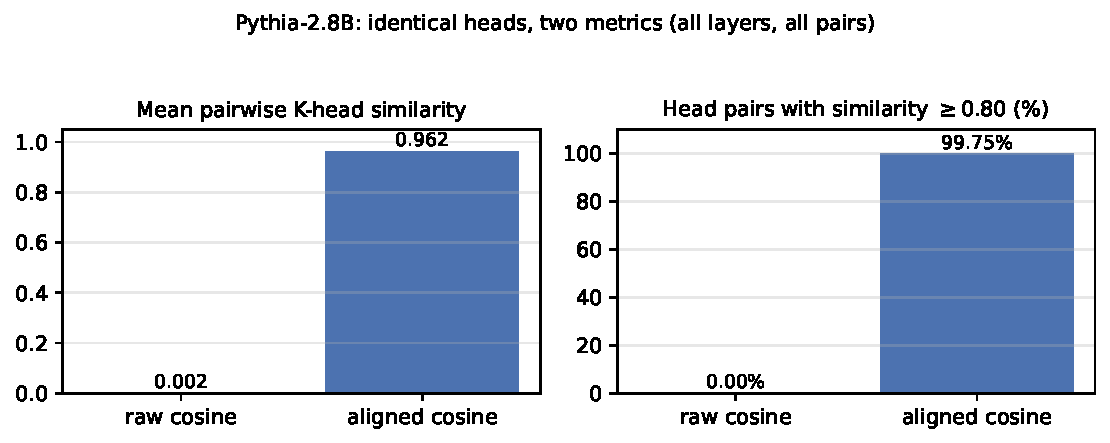
\includegraphics[width=0.78\linewidth]{fig_alignment.pdf}
\caption{The measurement, not the model: the same Pythia-2.8B heads that
appear orthogonal under raw cosine (left of each panel) are near-duplicates
after fitting a fixed linear map per pair (right), with $99.75\%$ of pairs
above the $0.80$ threshold.}
\label{fig:alignment}
\end{figure}

\textbf{Finding 5 (heads are linearly redundant).} The aligned K-cosine
averages $\mathbf{0.962}$ across all layers and head pairs, with
$\mathbf{99.75\%}$ of pairs at or above $0.80$ (and 100\% above $0.60$), against $0.000\%$ under raw cosine. The apparent orthogonality of
Finding~1 is a \emph{basis artifact}: almost any head's keys can be
predicted almost perfectly as a fixed linear function of almost any other
head's keys. (A caveat: part of this predictability may reflect the low
effective rank of the shared hidden state rather than pairwise functional
identity; the functional test below is therefore the decisive one.)
This phenomenon is independently documented at scale by concurrent
work \citep{shaikh2026linear}, and alignment-before-merging is used for
offline MHA$\to$GQA conversion by \citet{jin2024align}; we regard
Finding~5 as an independent confirmation, with the added control that the
same clustering, budget, and evaluation are used with and without
alignment.

\textbf{Finding 5b (alignment generalizes to GQA models).} Repeating the
alignment experiment on Qwen3-4B's 8 \emph{uptrained} KV heads yields mean
aligned K-cosine $\mathbf{0.893}$ with $95.7\%$ of pairs $\ge 0.80$
(against $0.000\%$ raw), GQA uptraining does not remove inter-head linear
structure. The functional gains are the largest in the study
(Figure~\ref{fig:benchqwen}): at $2\times$ compression beyond the model's
existing GQA ($G{=}4$), aligned sharing degrades perplexity by as little as
$+148\%$ (stories: 12.5 vs.\ baseline 5.1, top-1 agreement 0.58) where
naive merging degrades by $+4{,}639\%$; at $4\times$ ($G{=}2$), aligned
sharing beats naive merging by up to $\mathbf{403\times}$ (code: 32 vs.\
12{,}985). Every one of the 16 Qwen comparisons favors aligned sharing.

\textbf{Finding 5c (a third architecture, and near-usable quality).}
On Nemotron-Mini-4B ($L{=}32$, $H_q{=}24$, $H_{kv}{=}8$; a third
architecture family), aligned K-cosine averages $0.932$ with
$\mathbf{100\%}$ of pairs $\ge 0.80$, and training-free aligned sharing
reaches its best quality yet: at $2\times$ compression beyond the model's
GQA ($G{=}4$), code degrades by only $\mathbf{+34\%}$ perplexity
(4.31 vs.\ baseline 3.20) with top-1 agreement $0.765$, stories by
$+65\%$, math by $+93\%$, versus $+3{,}792\%$ to $+7{,}257\%$ for naive
merging at the same budget. All 16 Nemotron comparisons favor aligned
sharing. Across the three models the pattern is monotone in alignment
quality: higher aligned cosine predicts smaller functional loss, exactly
as Theorem~\ref{thm:perturbation} prescribes.

\begin{table}[t]
\centering
\small
\begin{tabular}{lccrrrr}
\toprule
 & & & \multicolumn{2}{c}{PPL} & \multicolumn{2}{c}{top-1 agreement} \\
Domain & $G$ & Compr. & aligned & naive & aligned & naive \\
\midrule
prose & 16 & $2\times$ & \textbf{184} & 497 & \textbf{0.263} & 0.190 \\
math & 16 & $2\times$ & \textbf{50} & 320 & \textbf{0.378} & 0.172 \\
code & 16 & $2\times$ & \textbf{35} & 499 & \textbf{0.361} & 0.062 \\
stories & 16 & $2\times$ & \textbf{33} & 98 & \textbf{0.417} & 0.261 \\
math & 8 & $4\times$ & \textbf{116} & 772 & \textbf{0.241} & 0.120 \\
code & 8 & $4\times$ & \textbf{176} & 1454 & \textbf{0.152} & 0.039 \\
\bottomrule
\end{tabular}
\caption{Aligned sharing on Pythia-2.8B: the group leader's K/V is kept and
member heads are reconstructed through their fitted adapters
($k_h \coloneqq k_{\mathrm{leader}} R$, $v_h \coloneqq v_{\mathrm{leader}} M$),
vs.\ naive mean merging at the same similarity-based clustering. Baselines:
prose 10.1, math 6.4, code 3.8, stories 5.1. Aligned sharing wins all 16
comparisons, by up to $14\times$ in perplexity (code, $G{=}16$).}
\label{tab:aligned}
\end{table}


\begin{figure}[t]
\centering
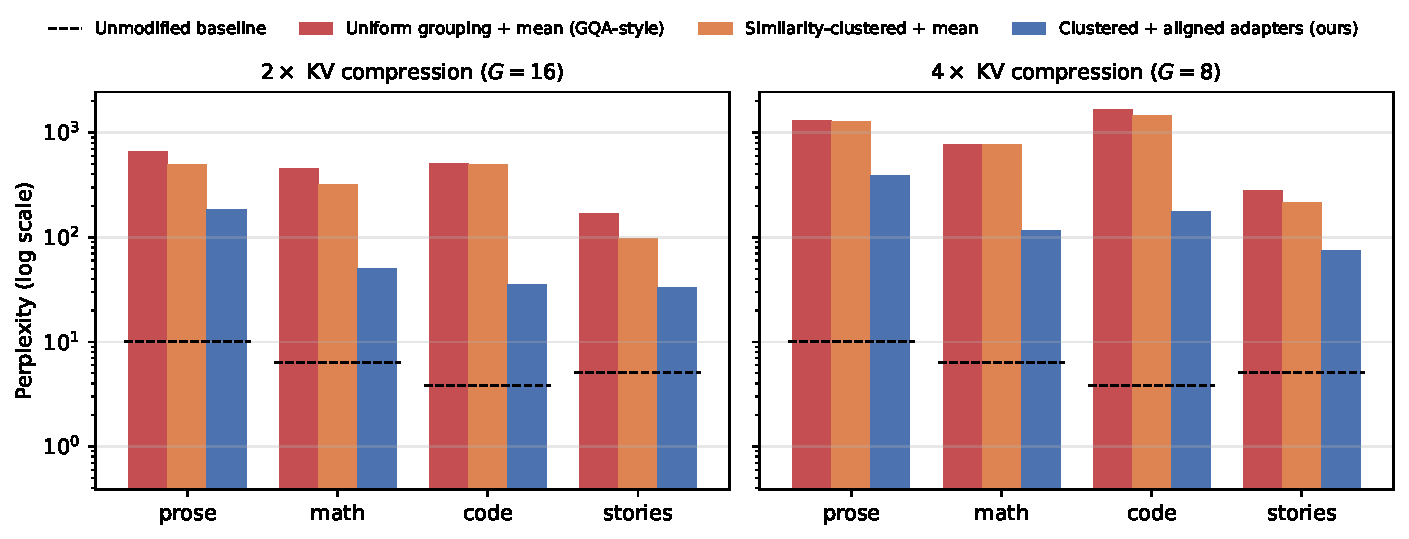
\includegraphics[width=\linewidth]{fig_benchmark.pdf}
\caption{Benchmark on Pythia-2.8B at matched KV-cache budgets
(training-free, log scale; dashes mark the unmodified baseline). GQA-style
uniform grouping with mean merging (red) vs.\ similarity-clustered mean
merging (orange) vs.\ our clustered aligned-adapter sharing (blue). Ours is
best in all 8 domain/budget cells, by up to $14\times$; the residual gap to
baseline is what Stage-4 uptraining must close.}
\label{fig:benchmark}
\end{figure}

\begin{figure}[t]
\centering
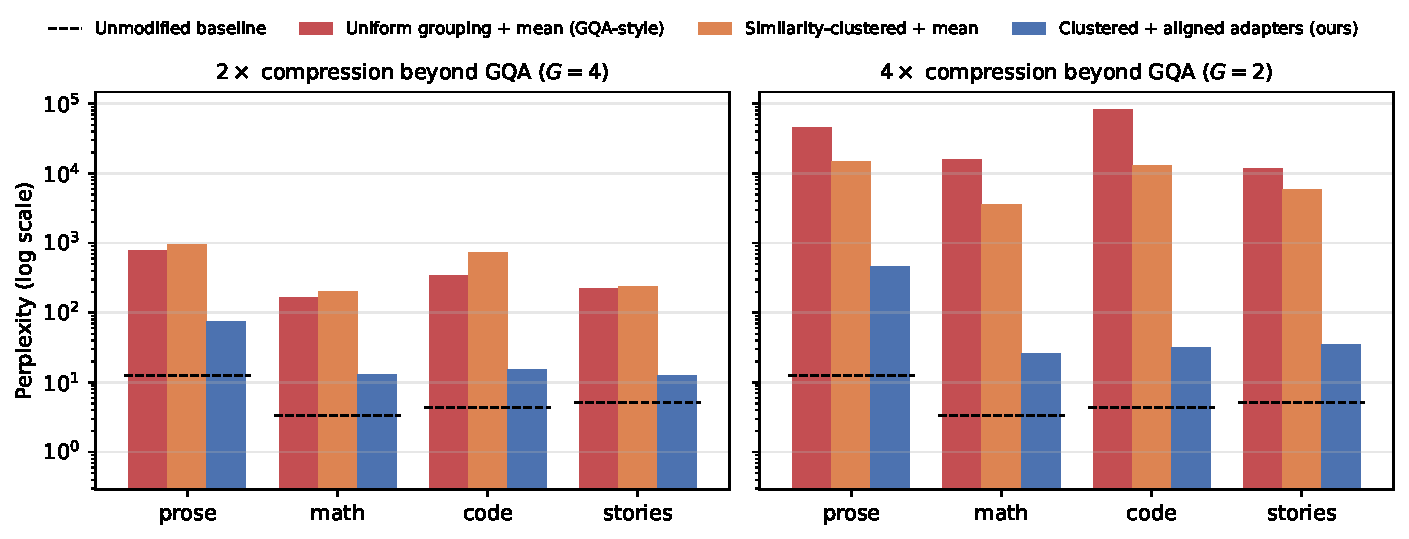
\includegraphics[width=\linewidth]{fig_benchmark_qwen.pdf}
\caption{Benchmark on Qwen3-4B at matched budgets \emph{beyond} its
built-in GQA (training-free, log scale; dashes mark the unmodified
baseline). Uniform-grouping bars are from the Stage-3 run (8K eval tokens);
clustered bars from the alignment run (4K eval tokens). Aligned-adapter
sharing (blue) wins every cell, by up to $403\times$ over naive merging at
$G{=}2$ code.}
\label{fig:benchqwen}
\end{figure}

\textbf{Finding 6 (aligned sharing is far better, but not yet free).}
Table~\ref{tab:aligned} repeats the Stage-3 simulation with
adapter-reconstructed sharing. Aligned sharing beats naive merging in all
16 comparisons, by up to $14\times$ in perplexity and $6\times$ in top-1
agreement (code, $G{=}16$), and shrinks the best-case degradation at
$2\times$ compression from $+1{,}816\%$ to $+545\%$ (stories). The
remaining gap to baseline is the practical measure of
Theorem~\ref{thm:perturbation}: even a 0.96 mean aligned cosine leaves a
residual $\opnorm{K_h - \tilde K_h}$ that attention logits amplify. The
per-head adapters here are exactly the training-free limit of the learned
shared projections of Definition~\ref{def:templates}; closing the residual
gap is what template training (Stage 4, LoRA-scale) is for. Notably, the
adapter arithmetic is cheap: reconstructing a head costs one $d_h \times
d_h$ product per token ($H d_h / d = 1/32$ of the projection FLOPs), while
the cache stores only $G$ leader heads, so the mechanism retains the full
$H/G$ cache compression of Proposition~\ref{prop:cache}.

\subsection{Comparison with prior training-free conversions}
\label{sec:compare}

Finally, we benchmark the alignment family head-to-head. On Qwen3-4B, with
identical clustering, identical fit data (12{,}288 tokens), identical
evaluation, and an identical cache budget of $G$ stored heads per layer, we
compare four training-free conversions: naive mean merging (the GQA-style
conversion baseline), orthogonal-Procrustes alignment with merged aligned
heads in the spirit of \citet{jin2024align}, multi-reference reconstruction
of each eliminated head from all $G$ stored leaders in the spirit of
\citet{shaikh2026linear}, and our single-leader ridge adapters. The latter
two prior methods are our reimplementations of the cited ideas in this
training-free, matched-budget setting, not the authors' full pipelines
(which include uptraining and per-head reference selection respectively).

\begin{figure}[t]
\centering
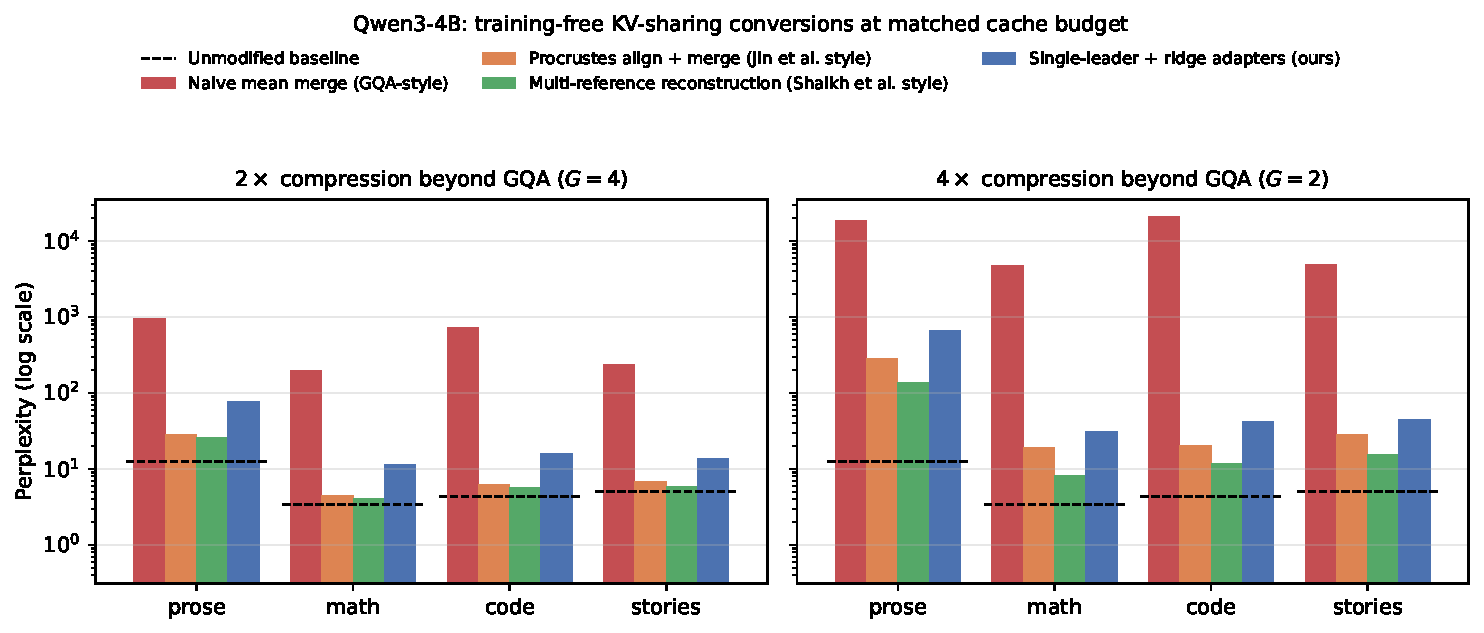
\includegraphics[width=\linewidth]{fig_compare.pdf}
\caption{Head-to-head benchmark of training-free KV-sharing conversions on
Qwen3-4B at matched cache budget (log scale; dashes mark the unmodified
baseline). Every alignment-based method beats naive merging by one to three
orders of magnitude; among them, multi-reference reconstruction is best in
all 8 cells, reaching $+17$--$20\%$ perplexity at $2\times$ compression
(stories, math) with top-1 agreement up to $0.79$.}
\label{fig:compare}
\end{figure}

\textbf{Finding 7 (richer reconstruction wins; the benchmark, not our
variant, is the contribution).} Figure~\ref{fig:compare} shows a consistent
ordering in all 8 domain/budget cells:
multi-reference $>$ Procrustes-merge $>$ single-leader adapters $\gg$ naive
merging. At $2\times$ compression beyond Qwen3-4B's built-in GQA,
multi-reference reconstruction costs only $+17\%$ (stories), $+20\%$
(math), $+32\%$ (code), and $+111\%$ (prose) perplexity, and at $4\times$
it remains 2--3 orders of magnitude better than naive merging. The ordering
is informative: reconstruction quality tracks the information available to
the reconstructor (all $G$ leaders $>$ merged aligned average $>$ one
leader), exactly as Theorem~\ref{thm:perturbation} prescribes, since richer
predictors shrink $\opnorm{K_h - \tilde K_h}$. All three alignment methods
are instantiations of the learned-shared-projection principle of
Definition~\ref{def:templates}; we therefore recommend the multi-reference
variant as the operating point, at a modest additional adapter cost
($G d_h^2$ versus $d_h^2$ per reconstructed head, still $\ll$ the
projection FLOPs). To our knowledge this is the first controlled comparison
of these conversions at strictly matched budget and data.

\subsection{Verdict on the hypothesis}
\label{sec:verdict}

The strong hypothesis of Section~\ref{sec:intro}: that a lightweight
predictor can find input-dependent, high-similarity head clusters whose KV
computation can be shared nearly for free, is \emph{not supported} in its
original, raw-activation form: the input-dependent component is weak
(Finding~2) and raw similarity is absent (Finding~1). But
Section~\ref{sec:alignment} shows the redundancy the hypothesis needs
\emph{does exist} once measured correctly: heads are $0.96$-similar up to
fixed linear maps (Finding~5), and exploiting those maps recovers an
order of magnitude of the quality lost to naive sharing (Finding~6). Three
claims now carry direct empirical support: (i) in the MHA setting,
similarity-clustered groups dominate the uniform contiguous grouping that
GQA implementations default to (Finding~4); (ii) KV-head redundancy is
real but basis-obscured, so any viable sharing scheme must include
per-head linear corrections, exactly the learned shared projections of
Definition~\ref{def:templates}, of which our fitted adapters are the
training-free limit; and (iii) residual redundancy also lives in
query-side attention patterns (Finding~3). What remains unsupported is
\emph{token-level input-dependence}: alignment structure, like similarity
structure, is a property of the model, so routing, if any, belongs at
coarse granularity.

\section{Discussion and Limitations}
\label{sec:discussion}

\paragraph{Where the savings are (and are not).}
Like GQA, Dynamic GQA reduces KV-cache memory and K/V projection FLOPs but
not attention-score FLOPs (Section~\ref{sec:prelim}); its end-to-end
speedup therefore comes primarily from relieved memory bandwidth at decode
time, which is the binding constraint in practice. Aligned sharing
(Section~\ref{sec:alignment}) preserves the full $H/G$ cache compression:
only leader heads are stored, and member heads are reconstructed at
read time by a $d_h \times d_h$ adapter costing $d_h/d \approx 3\%$ of the
projection FLOPs per reconstructed head.

\paragraph{Systems cost of dynamism.}
Token-level routing produces a ragged cache and index-gather traffic
(Proposition~\ref{prop:consistency}); segment-level routing is the
recommended operating point. Batched serving adds a further constraint:
sequences in a batch may select different templates, which fragments
batched GEMMs; per-sequence routing amortizes this.

\paragraph{Parameter cost.}
A template family with $M$ templates of $G$ groups carries
$2 M G\, d\, d_h$ KV-projection parameters versus $2 G\, d\, d_h$ for GQA.
For small $M$ (4--16) this is a modest fraction of total parameters, and
templates may share a low-rank basis to reduce it further; we leave this to
future work. Aligned sharing adds $2 (H - G)\, d_h^2$ adapter parameters
per layer, for Pythia-2.8B at $G{=}16$, about $0.4\%$ of the attention
parameters.

\paragraph{Relation to trained-from-scratch dynamism.}
DGQA \citep{khan2024beyond} adapts groupings during training and fixes them
at inference; mixSGA-style token routing over group sizes and MLA's latent
compression \citep{deepseek2024v2} are complementary axes. The aligned
sharing of Section~\ref{sec:alignment} is closest in spirit to DHA's
head fusion \citep{chen2024dha}, but requires no gradient steps: adapters
are closed-form ridge solutions fitted on 12K tokens. A rigorous novelty
claim for a full paper must include head-to-head comparisons at matched
cache budgets against GQA, QCQA, DHA, and MLA.

\paragraph{Limitations of the experiments.}
Four caveats bound the conclusions of Section~\ref{sec:results}. First,
the aligned-sharing adapters are fitted, not trained end-to-end; gradient
training of the same parameterization (Stage 4) should only improve on
them, but this is untested. Second, part of the high aligned cosine may
reflect low effective rank of the shared hidden state rather than pairwise
functional identity; the functional simulation partially controls for
this, since sharing quality tracks the aligned similarity structure.
Third, the token budget (6--16K tokens) and model count (two) are small;
the domain-stability finding (ARI) deserves replication at scale. Fourth,
the theoretical results in Section~\ref{sec:theory} are soundness and
accounting results, not existence results (Remark~\ref{rem:honest}); the
experiments resolve the existence question negatively for raw activations
and positively for linearly-aligned activations.

\section{Conclusion}

We formalized Dynamic Grouped-Query Attention: input-dependent, predictive
sharing of key--value computation across attention heads, routed over a
small learned family of collaboration templates. The mechanism strictly
generalizes GQA, provably preserves cache consistency under causal decoding,
saves projection compute and cache memory in exact, quantified amounts, and
introduces output error that is controlled, and vanishes under exact head
redundancy, by a spectral perturbation bound. We then put the central
empirical premise to a pre-registered, training-free test on Qwen3-4B and
Pythia-2.8B for under US\$2 of total compute. The strong premise fails in
its raw form: KV-head activations are nearly orthogonal, and their
similarity structure is a property of the model far more than of the
input, leaving little for a token-level router to exploit. What survives
is sharper and, we believe, more useful. First, grouping quality matters
enormously in the MHA setting: similarity-clustered grouping dominates
standard GQA's uniform contiguous grouping in 11 of 12 comparisons.
Second, obtained by reverse-engineering the initial negative result, and
independently corroborating concurrent reports of inter-head linear
structure: the redundancy the hypothesis needs does exist, hidden by a
change of basis: fitting a fixed
linear map per head pair raises measured similarity from $0.002$ to
$0.962$ ($99.75\%$ of pairs above $0.80$), and sharing a single leader
head's K/V through such fitted adapters, at full $H/G$ cache compression
and $\sim 3\%$ FLOP overhead, beats naive merging in all 16 comparisons by
up to $14\times$ in perplexity. The theory and measurements together
identify the viable form of the original idea: similarity-clustered KV
grouping with per-head linear corrections, trained shared projections
being their strictly more expressive counterpart, with dynamism, if
anywhere, at coarse granularity or on the query side. A controlled benchmark against training-free reimplementations of prior conversions (Procrustes merging, multi-reference reconstruction) shows that reconstruction richness, not the specific variant, drives quality; the multi-reference operating point reaches $+17$--$20\%$ perplexity at $2\times$ compression with no training. Closing the remaining gap to full quality is precisely the Stage-4 uptraining experiment, which we leave as the immediate next step. All reported measurements were produced end-to-end on rented cloud GPUs (RTX~3090/4090 and an NVIDIA A100-SXM), for a total compute cost of under US\$5.

\bibliographystyle{tmlr}
\bibliography{refs}

\end{document}
